\subsection*{B1}
    \subsubsection*{Les besoins qui ont mené à l'émergence des containers}
        Le besoin d'une solution technique telle que les containers provient de plusieurs demandes:
        \begin{itemize}
            \item \textbf{La simplification de la configuration}: la plupart des applications sont déployées dans le cloud aujourd'hui, et les entreprises peuvent être amenées à changer de fournisseur d'infrastructure (IaaS) ou de plateforme (PaaS) durant leur vie. Ceci est en partie possible grâce aux machines virtuelles, mais leur consommation de ressources est très importante et la répétabilité de la construction de telles machines n'est pas souvent aisée;
            \item \textbf{Un environnement constant dans la chaîne de livraison}: de la machine d'un développeur à la production, le code s'exécute dans plusieurs environnements, parfois chez différents prestataires. Chaque environnement (développement, test, QA, staging, production\dots) possède sa part de changements mineurs qui peuvent avoir un impact sur le comportement de l'application finale. Ici le besoin est une infrastructure immutable, que l'on peut reproduire facilement;
            \item \textbf{Productivité des développeurs}: les développeurs ont besoin de deux choses principales : avoir un environnement de travail le plus proche possible de la production et pouvoir travailler rapidement dans un tel environnement, sans passer des heures à configurer des composants. Ceci permet à ce que des développeurs moins à l'aise avec l'administration système puissent effectuer leur travail et permet d'éliminer la difficulté de la mise en place d'un environnement de travail pour une nouvelle recrue;
            \item \textbf{Isolation des applications}: il arrive parfois que des applications doivent fonctionner en même temps et qu'elles utilisent les mêmes technologies, mais dans des versions différentes. Le besoin d'isolation se fait alors ressentir, pour éviter ce que l'on appelle souvent le \enquote{\textit{dependency hell}};
            \item \textbf{Gestion des ressources}: les machines virtuelles ont souvent été très efficaces pour déployer plusieurs composants sur un serveur physique hôte puissant. Toutefois, leurs consommations en ressources restent importantes et les ressources non utilisées ne peuvent pas être allouées à d'autres machines virtuelles, qui auraient besoin de plus de ressources au même moment;
            \item \textbf{Rapidité de déploiement}: auparavant, mettre en place un nouveau serveur physique et le configurer prenait plusieurs heures. La virtualisation a réduit ce temps à l'ordre de quelques minutes mais le besoin de réduire ce temps est encore présent. En effet l'utilisation de services est variable en fonction de la demande et parfois les ressources non utilisées pourraient ne pas être payées dans le cas d'IaaS ou de PaaS. Ces ressources non utilisées par la production pourraient également être affectées à la réalisation de tâches non urgentes, peu gourmandes ou longues en temps d'exécution. On retrouve ce besoin de changement d'échelle et d'affectation de ressources, avec une demande de réactivité et de rapidité d'exécution.
            \item \textbf{Versionnage et partage de l'infrastructure}. Les gestionnaires de version sont désormais habituels dans le monde de l'ingénierie logicielle. Se pose alors la question: pourquoi n'est-il pas possible de pouvoir partager des éléments d'infrastructure, de description des composants, des services des paquets dans des fichiers de configuration. On parle souvent d'\enquote{\textit{Infrastructure as code}}. Comme pour les gestionnaires de version, l'envie de pouvoir télécharger des descriptions d'infrastructure créées par d'autres personnes se faire sentir, pour éviter que chacun ne réinvente la roue de son côté.
        \end{itemize}

     \subsubsection*{Approche technique des containers}
        Pour répondre au besoin de déploiement rapide et à la consommation faible en ressources, les containers prennent le contre pied des pieds virtuelles et ne cherchent pas à reproduire une machine physique.\\

        Les machines virtuelles permettent de simuler une machine physique et donc de faire tourner une application de très bas niveau à savoir un système d'exploitation de son choix. Grâce à cela, une machine physique sous un système d'exploitation peut faire tourner plusieurs machines virtuelles avec chacun son propre système d'exploitation et son ensemble applicatif. Cette solution est relativement performante si elle repose sur des fonctions matérielles (architecture physique compatible et si possible avec instruction AMD-V, VT-d, VT-x\dots) car sinon il faut opérer par émulation (perte de près de 50\% des performances CPU lors d'émulation de x86 sur PowerPC)\cite{ipponDocker}. Les machines virtuelles sont souvent considérées comme sécurisées car il n'y a pas de communication directe entre machine virtuelles et la machine hôte.\\

        Un conteneur virtualise l'environnement d'exécution du système d'exploitation de la machine hôte (Linux ou BSD, il n'existe pas à ce jour de conteneur sous Windows). Un conteneur est un ensemble applicatif s'exécutant au sein du système d'exploitation maître de manière virtuellement isolée et contrainte. Le conteneur est très performant et léger car il partage de nombreuses ressources avec le système d'exploitation hôte (kernel, devices\dots). En revanche bien que s'exécutant de manière isolée, le conteneur ne peut être considéré comme très sécurisé puisque partageant la stack d'exécution avec le système d'exploitation maître. Le conteneur peut au choix démarrer un système d'exploitation complet ou bien simplement des applications. D'autres outils utilisant des containers tel qu'OpenStack ou Proxmox gèrent des containers pour virtualiser tout le système d'exploitation.\\

        Pour que la configuration et le partage de ces containers soient pratiques, la description du contenu d'un conteneur est souvent réalisée dans un fichier texte. Un programme est alors requis pour créer un conteneur à partir du fichier. L'utilisation d'un fichier texte de description d'un conteneur facilite le versionnage de celui-ci dans un gestionnaire de version. Les logiciels de containers proposent souvent des annuaires de container, où la communauté open source peut partager des containers déjà créés, que l'on peut configurer avec ses besoins par la suite. Ceci correspond à la mise en place du pattern \enquote{Partage d'images}.\\

        Il est possible de créer totalement un conteneur mais la plupart des logiciels de conteneurs propose un système d'héritage, qui permet aux utilisateurs de créer un conteneur reprenant le template de base d'un conteneur dit \enquote{de base}. Ceci correspond à la mise en place du pattern \enquote{conteneur de base}. L'utilisation des conteneurs de base est conseillée, puisqu'elle permet de simplifier les fichiers de description du conteneur. Il est également conseillé de séparer autant que possible différentes fonctionnalités dans différents conteneurs, ce qui rejoint l'idée des patterns \enquote{conteneur d’outils de développement} et \enquote{conteneur dédié au build}.\\

        La plupart des logiciels de conteneurs implémente le pattern d' \enquote{Utilisation du cache lors du build}, qui permet de réduire le temps de construction des conteneurs en réutilisant des parties des images existantes.\\

        Enfin, même s'il est souvent possible de définir quelques éléments de configuration dans les containers (système d'exploitation, paquets à installer, utilisateurs à créer), ceux-ci ne cherchent pas à remplacer des gestionnaires de configuration comme Chef, Puppet ou Ansible qui offrent bien plus de possibilités.

\subsection*{B2}

    \subsubsection*{Docker}
    Docker est un logiciel libre qui automatise le déploiement d'applications dans des conteneurs logiciels. Selon la firme de recherche sur l'industrie 451 Research, « Docker est un outil qui peut empaqueter une application et ses dépendances dans un conteneur virtuel, qui pourra être exécuté sur n'importe quel serveur Linux ».\\

    La technologie de conteneur de Docker peut être utilisée pour étendre des systèmes distribués de façon à ce qu'ils s'exécutent de manière autonome depuis une seule machine physique ou une seule instance par nœud. Cela permet aux nœuds d'être déployés au fur et à mesure que les ressources sont disponibles, offrant un déploiement transparent et similaire aux PaaS pour des systèmes comme Apache Cassandra, Riak ou d'autres systèmes distribués.

    \subsubsection*{Kubernetes}
    Google est derrière Kubernetes, un gestionnaire open source de conteneurs. Ce dernier permet de déployer des conteneurs sur un lot de machines, d’en surveiller le bon fonctionnement et d’assurer leur réplication. Une offre idéale pour administrer des conteneurs Linux sur une infrastructure de type cloud public. Microsoft s'est assuré que Kubernetes fonctionne bien sur Azure, Red Hat a fait de même. Docker et CoreOS assurent également la compatibilité avec Kubernetes et se sont engagés à assurer la compatibilité dans le futur, avec l'aide entre autre d'IBM.

    \subsubsection*{OpenVZ}
    OpenVZ est un système de virtualisation pour Linux basé sur des conteneurs. OpenVZ permet à un même serveur physique de faire tourner plusieurs instances, isolées, d'un système d'exploitation. Tous les conteneurs OpenVZ doivent alors partager la même architecture et la même version de kernel. Ainsi cette méthode de virtualisation offre de meilleures performances et un meilleur changement d'échelle que ses concurrents classiques de virtualisation tels que VMware, n'utilisant pas la notion de conteneurs.

    \subsubsection*{runC}
    RunC est un outil de lignes de commandes permettant de créer et de lancer des conteneurs. RunC implémente le standard OCF (Open Container Format). C'est un wrapper autour de libcontainer, qui a été donné par Docker au Open Container Project afin de servir d'implémentation de référence. RunC peut faire tourner des images de Docker sans lancer de deamon Docker.


    \subsubsection*{Choix de deux solutions}
    Les solutions que nous avons choisies pour la suite du projet sont Docker et runC.

\subsection*{B3}
    Une description générale de Docker et runC a déjà été effectuée dans les parties A4 et B2.\\

    Docker et runC fonctionnent tous les deux à l'aide de fichiers textes de configuration, ce qui facilite le partage et le versionnage des outils de travail. Ces deux logiciels supportent l'héritage: c'est-à-dire que l'on peut créer un nouveau conteneur à partir d'un conteneur parent. Docker propose de partager des images de conteneurs déjà construits et configurables sur Docker Hub. Ces images peuvent être alors être téléchargées, étendues ou configurées pour répondre aux besoins. Les deux outils possèdent également un système d'utilisation du cache lors du build.

\subsection*{B4}
    Les métriques retenues pour comparer les deux solutions choisies sont:
    \begin{itemize}
        \item Number of failures (correspondant aux facteurs qualité Resource utilization et Fault tolerance)
        \item Operation time (correspondant au facteur qualité Resource utilization)
        \item CPU (correspondant au facteur qualité Resource utilization)
        \item Number of installation steps (correspondant au facteur qualité Installability)
        \item Number of setup operations (correspondant au facteur qualité Installability)
        \item Number of step / number of setup operations = number of steps by setup operation (correspondant au facteur qualité Installability)
        \item Number of test cases (correspondant au facteur qualité et Fault tolerance)
        \item Number of failure + Number of breakdowns x 10 (correspondant au facteur qualité et Fault tolerance)
    \end{itemize}

\subsection*{B5}

    \begin{figure}[H]
            \centering
            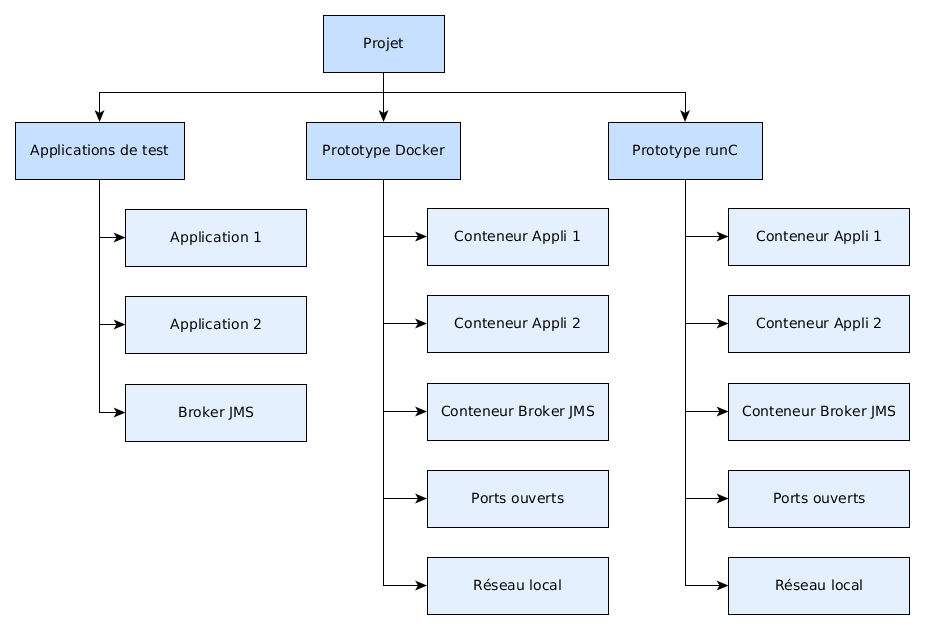
\includegraphics[width=\textwidth]{images/WBS.png}
            \caption{Work Breakdown Structure pour la réalisation des prototypes}
            \label{fig:wbs}
    \end{figure}
